\label{Jonas}
Um sich einen Überblick über die Thematik verschaffen zu können, wurden verschiedene Self-Assessment-Tests anderer Universitäten analysiert.
Hierbei ist wichtig zu wissen, dass folgende Beschreibungen sich nur auf die jeweiligen Benutzeroberflächen der Tests beziehen.

\subsection{Test der Universität Frankfurt}
Der Test
\footnote{\url{https://www.gdv.informatik.uni-frankfurt.de/selfassessment/Informatik/}} 
der Universität Frankfurt beginnt mit einem Motivationstext, der sowohl Sinn und Zweck des Tests erklärt, als auch den User in die Benutzung einführt.

Desweiteren wird angeboten den Test der Universität Frankfurt herunterzuladen, was eine Offline-Bearbeitung realisiert. 
Bei unserem Test wird der aktuelle Zustand in der URL der Webseite kodiert. 
Dies ermöglicht zwar keine Bearbeitung ohne Internet, bietet aber an, den Test jederzeit zu pausieren, indem man sich die URL abspeichert.

Der zu vergleichende Test erfordert außerdem eine persönliche Registrierung, welche sehr ausführlich ist, was dazu führt, dass die Benutzererfahrer sinkt. Daher wurde eine Registrierung in unserem Test weggelassen, um die Flexibilität und Einfachheit zu gewährleisten.  
\begin{figure*} 
  \centering
     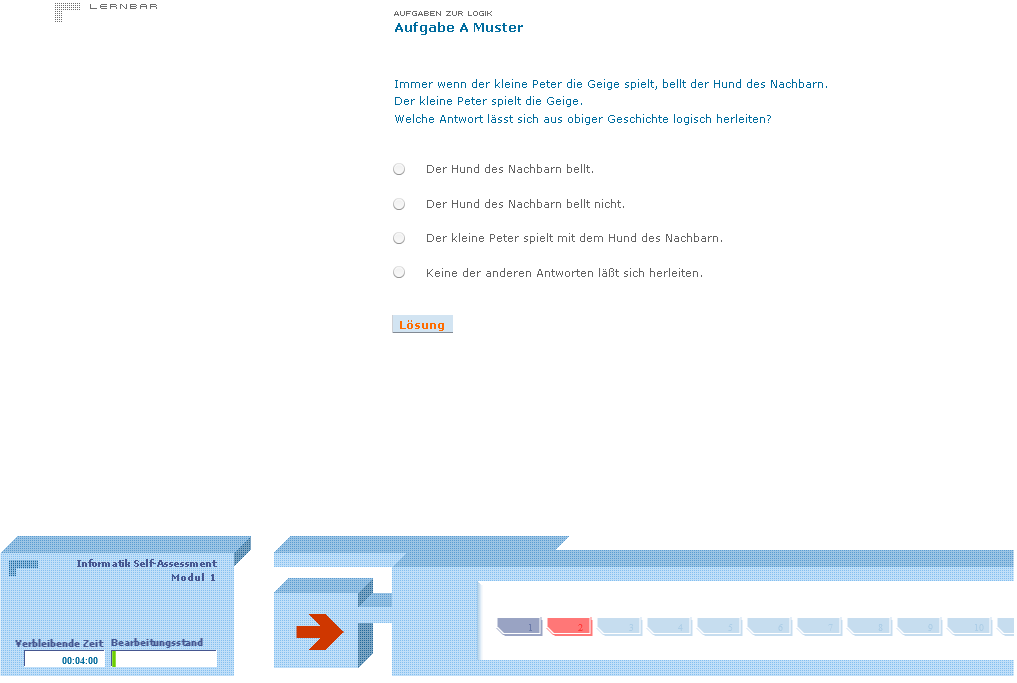
\includegraphics[width=\textwidth]{Jonas_Images/frankfurt1.png}
  \caption{}
  \label{fig:Bild1}
\end{figure*}
In Abbildung~\ref{fig:Bild1} ist das Grundlayout des Tests von der Universität Frankfurt zu sehen. 
Das Layout ist sehr ähnlich zu unserem und beinhaltet die Frage mit ihren Antworten, einen Fortschrittsbalken, einen Next-Button und eine Zeitanzeige.

Auch ist es möglich Grafiken anzeigen zu lassen.
Der Test wird in verschiedene Kategorien eingegliedert, die wiederholbar sind. 
Bei unserem Test ist die Erstellung von Kategorien ebenfalls möglich, ein Mehrfachbeantwortung ist jedoch ausgeschlossen.

Abschließend bietet der Test der Universität Frankfurt eine Bewertung der beantworteten Fragen.
Anders als die Universität Frankfurt enthält unser Test insbesondere eine persönliche Beurteilung des Erstellers.
Diese diehnt als Abschließendes Feedback für die erbrachte Leistung des Nutzers im Test.

\subsection{Test der RWTH Aachen}
\begin{figure*}[htbp] 
  \centering
     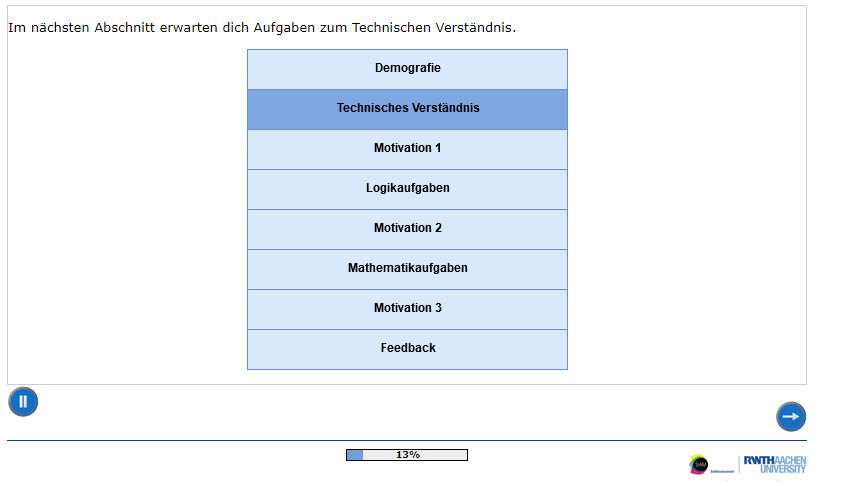
\includegraphics[width=0.5\textwidth]{Jonas_Images/Abschnitte.png}
  \caption{}
  \label{fig:Bild4}
\end{figure*}
Der Test der RWTH Aachen \footnote{\url{https://www.global-assess.rwth-aachen.de/rwth/tm_alt/}} ähnelt unserem Ansatz, wie man in Abbildung \ref{fig:Bild4} sehen kann.
Das Layout ist einfach gehalten und überschaubar. 
Es gibt einen Next-Button und einen Fortschrittsbalken.
In beiden Ansätzen besteht keine Möglichkeit, eine Frage zu überspringen.
Außerdem bedarf es einer Anmeldung, um am Test der Hochschule Aachen teilnehmen zu können.
Damit die Hemmschwelle zur Teilnahme möglichst niedrig gehalten wird, haben wir dafür entschieden, auf jede Form der Anmeldung zu verzichten.



